
During the dedicated experiment that took place in the SPS
in 2018 with the CCs, the measured emittance
growth was found to be a factor four (on average) lower than
expected from the theory (see Section~\ref{sec:meas_2018_vs_theory}). The reason for this discrepancy remained unresolved for some time, as detailed follow-up studies (see Chapter~\ref{Ch:investigating_discrepancy}) investigated and excluded a number of possible explanations for the discrepancy.
It was recently found, that the beam transverse impedance, which is not included in the theory~\cite{PhysRevSTAB.18.101001} used for the comparison with the measurements may impact the noise-induced emittance growth and explain the experimental observations. Here, the damping mechanism from the beam transverse impedance is investigated as observed in detailed PyHEADTAIL simulations.

The structure of this chapter is as follows:




\section{SPS transverse impedance model}\label{sec:sps_impedance_model}
The PyHEADTAIL studies presented in this chapter are performed including the detailed transverse impedance model of the SPS machine~\cite{sps_impedance_model_git}. This model has been developed through a combination of theoretical computations, electromagentic simulations and was benchmarked with beam-based measurements~\cite{Salvant:1274254, Zannini:1561199, Salvant:1271349, Zannini:2141779}. 
It includes the contributions from all the individual elements in the SPS lattice i.e. the resistive wall, the indirect space charge, the kickers, the RF cavities (200\,MHz and 800\,MHz), the step transitions and the horizontal and vertical beam position monitors~\cite{Zannini:2141779}. As discussed in  Section~\ref{subsec:pyheadtail}, the model needs to represent the global impedance of the full machine. Thus, the total impedance is obtained by summing up the impedance of each element weighted with the beta function at its location and by dividing the sum by the average beta function of the SPS. For the Q26 optics the average horizontal and vertical beta functions are 42.09\,m and 42.01\,m respectively.
%https://indico.cern.ch/event/299470/contributions/686509/attachments/564150/777102/LIUSPS_transverse_imp_5.pdf
% The Wall contribution included both the resistive wall and the indirect SC.
Figure~\ref{fig:sps_impedance_model_H_V} shows the complete transverse impedance model of the SPS machine with the disentangled dipolar (blue) and quadrupolar (orange) terms to be plotted seperetaly. 

% Plot figures: /eos/user/n/natriant/Project_thesis/plot_wakefields_impedances_SPS
\begin{figure}[!ht]
    \centering
    \begin{subfigure}[t]{0.45\textwidth}
        \centering
        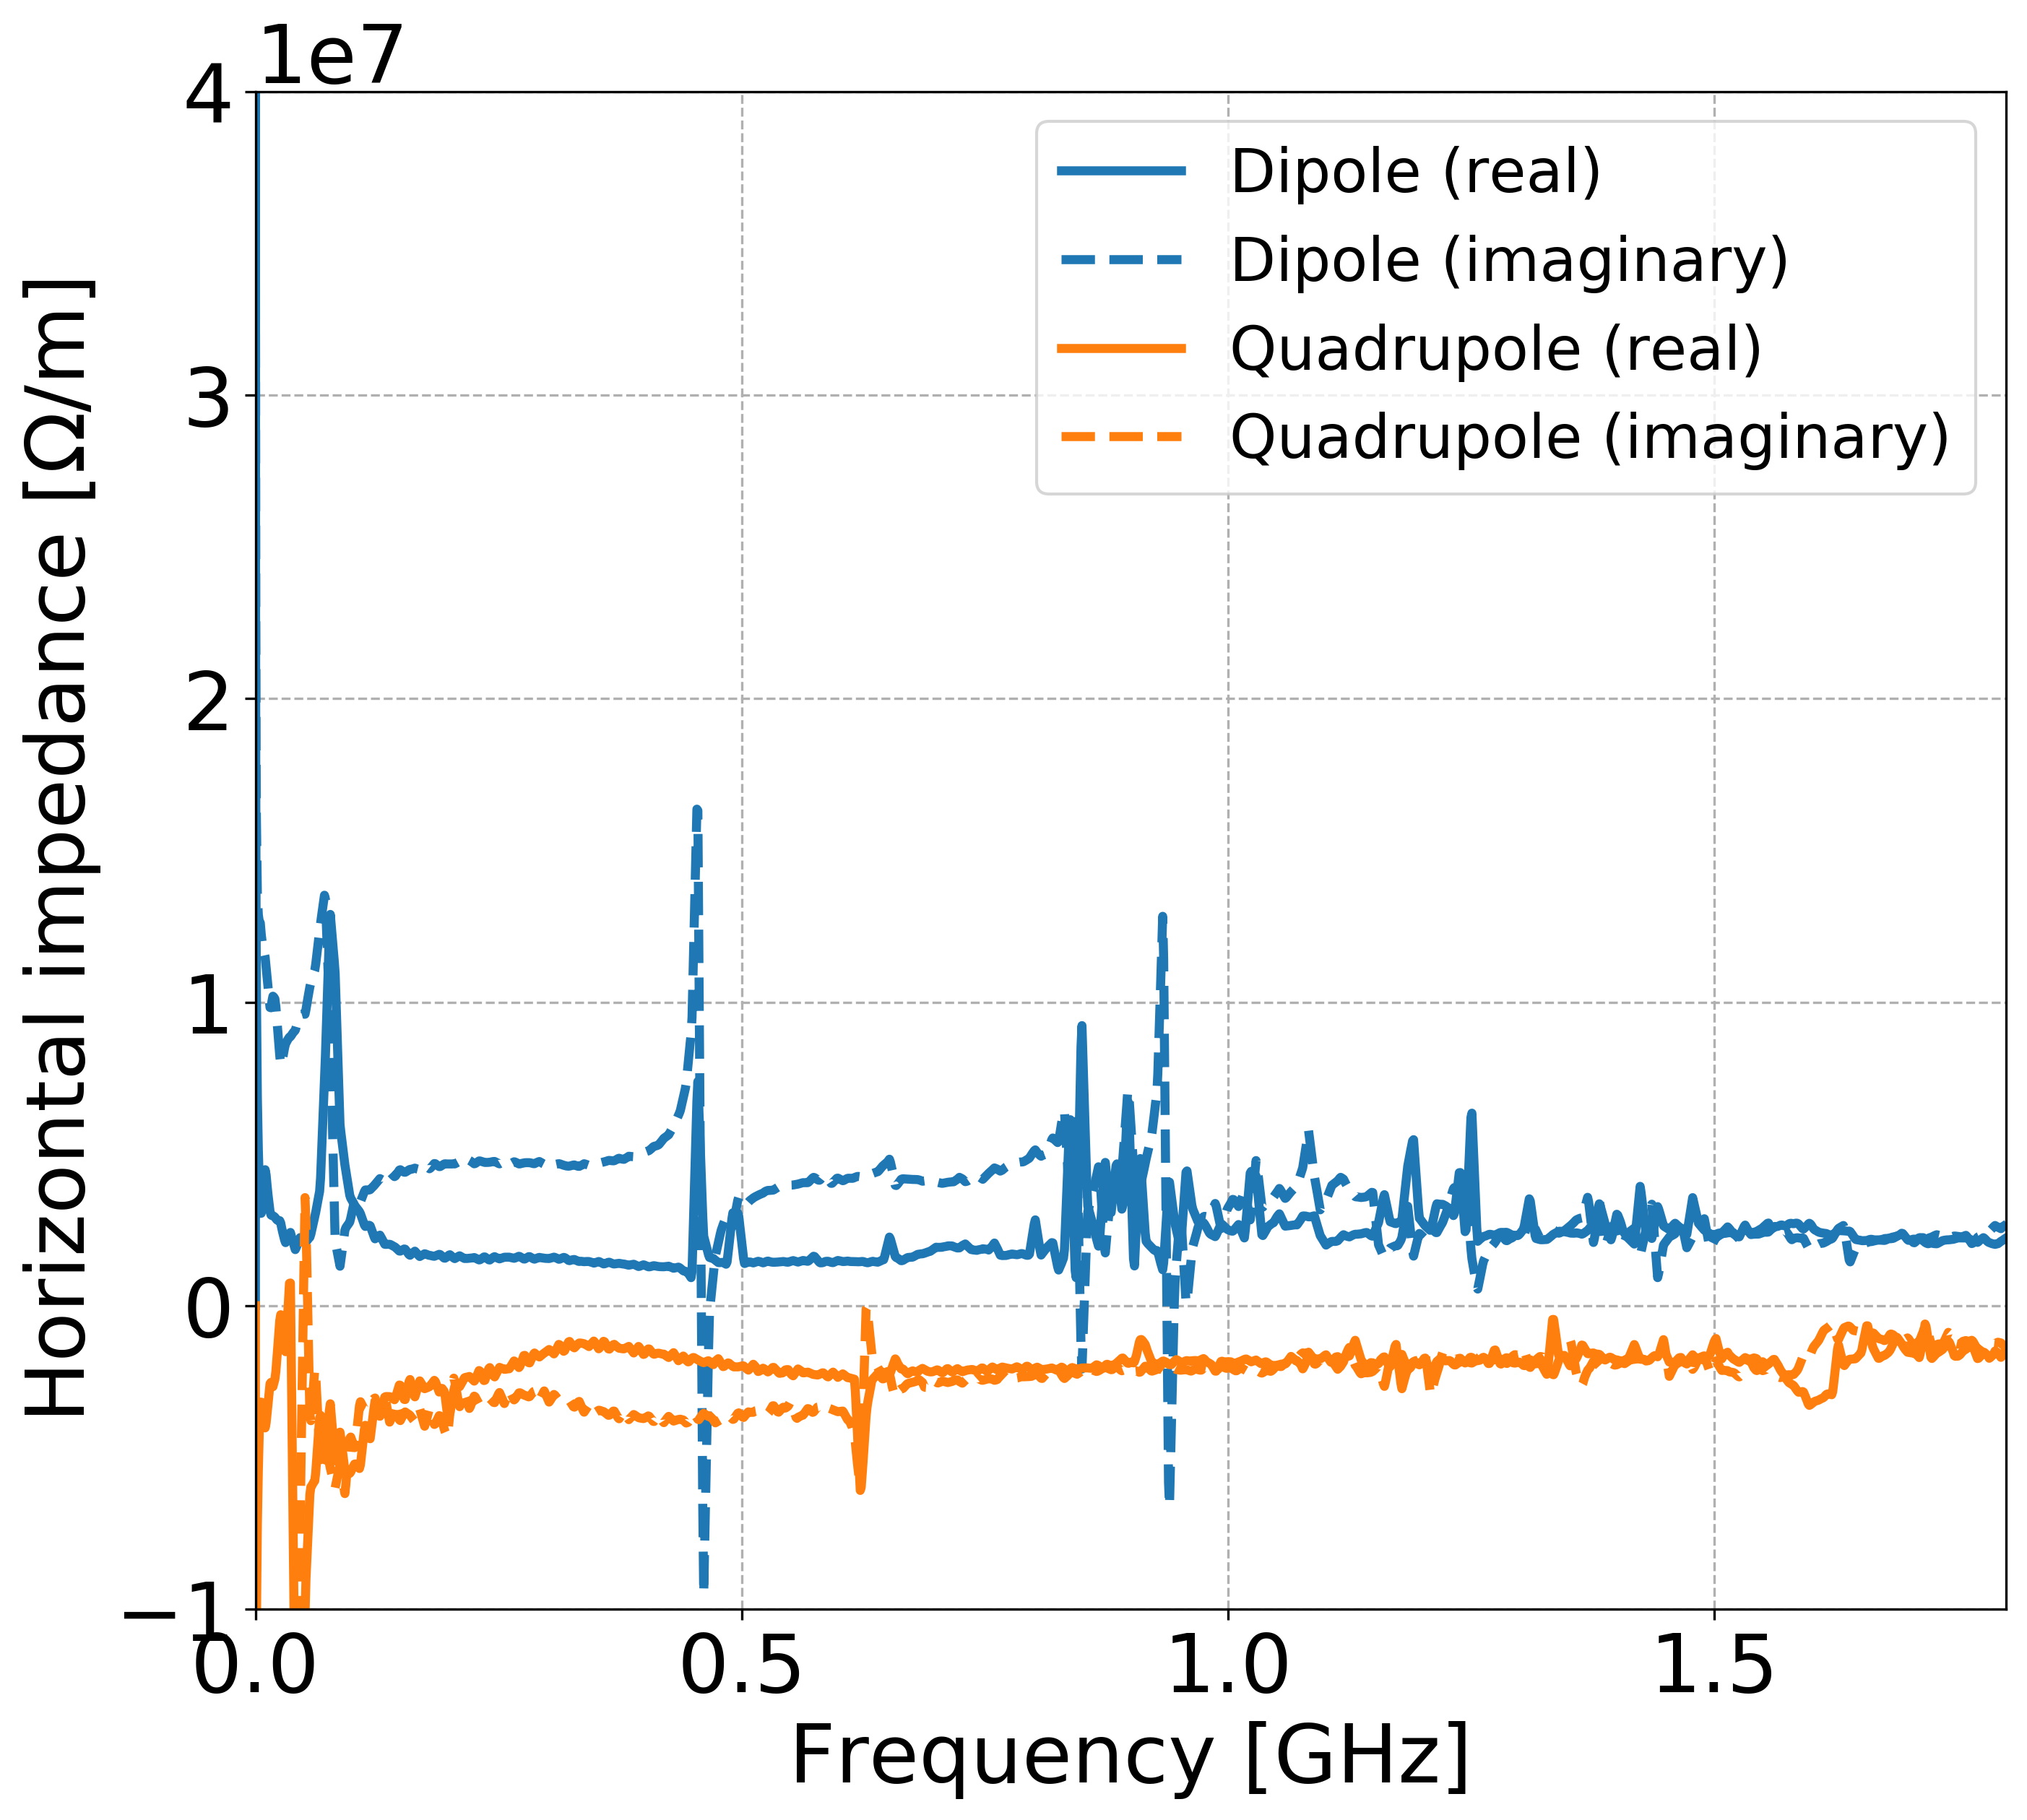
\includegraphics[width=1\textwidth]{images/Ch7/Q26_complete_SPS_model_impedance_H_plane.png}
        %\caption{$y=\sin(2 \pi f t),\ f=50$ Hz}
        %\label{fig:add_label_here}
    \end{subfigure}
    \hfill
    \begin{subfigure}[t]{0.45\textwidth}
        \centering
        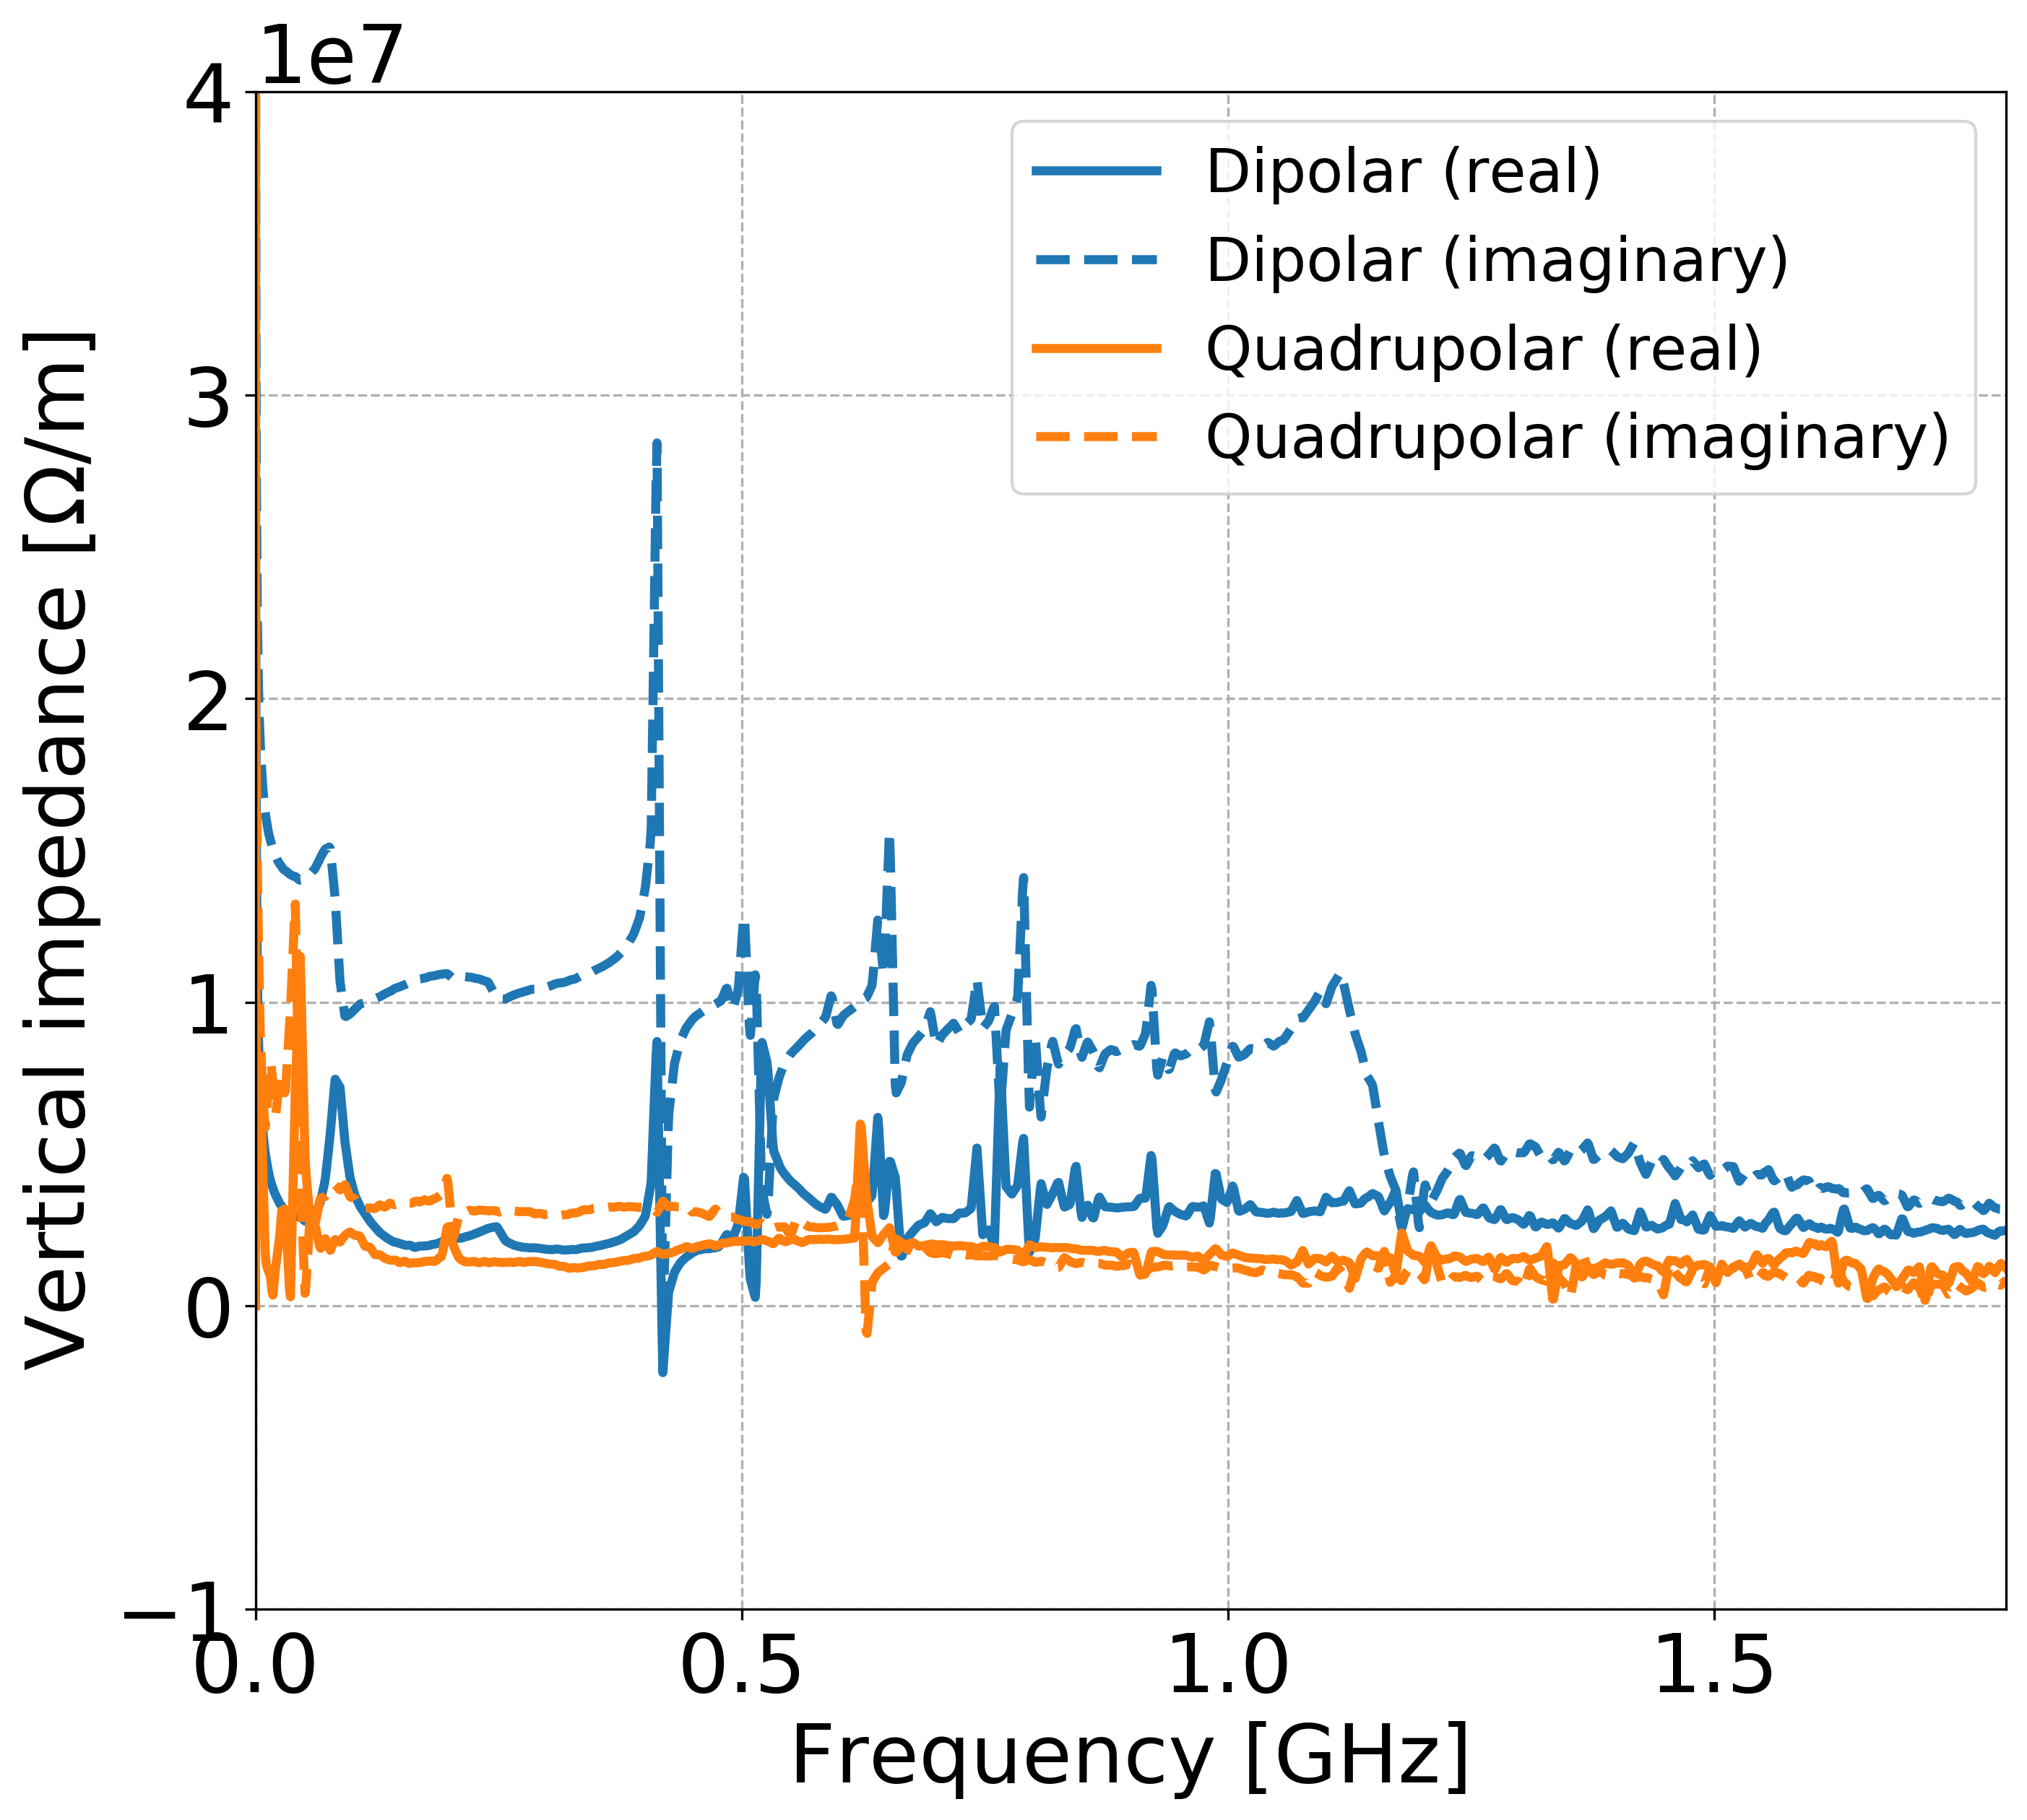
\includegraphics[width=1\textwidth]{images/Ch7/Q26_complete_SPS_model_impedance_V_plane.png}
        %\caption{Discrete Fourier transform}
        %\label{fig:add_label_here}
    \end{subfigure}
    \hfill
     \caption{Horizontal (left) and vertical (right) impedance model of the SPS. The model is available in the public gitlab repository of Ref.~\cite{sps_impedance_model_git}.} % bunch passage
     \label{fig:sps_impedance_model_H_V}
 \end{figure}

 The contributions from the wall, the kickers and the step transitions are visible at the low freqencies (up to $\sim$ 0.4\,GHz). The impedance of the RF cavities and the beam position monitors (BPMs) corresponds results to the peaks observed between $\sim$ 0.4-1\,GHz. 
%https://indico.cern.ch/event/299470/contributions/686509/attachments/564150/777102/LIUSPS_transverse_imp_5.pdf %For a clearer picture, it is worth mentioning that at low freqencies (up to $\sim$ 0.4\,GHz) the impedance is mainly from the wall the kickers and the step transitions. The peaks between $\sim$ 0.4-1\,GHz appear due to the RF cavities and the beam position monitors.
%https://indico.cern.ch/event/299470/contributions/686509/attachments/564150/777102/LIUSPS_transverse_imp_5.pdf

\normalsize{\textbf{Wake functions}}\\
As already discussed in Section~\ref{subsec:pyheadtail}, in order to include the impedance effects in PyHEADTAIL simulations the real-value wakefields in time domain are used. The wakefield kicks are computed as a convolution of the wake function with the moments of each particle. The total transverse dipolar (blue) and quadrupolar (orange) wake functions for both planes of the SPS can be found in the gitlab repository of Ref.~\cite{sps_impedance_model_git} and they are plotted in Fig~\ref{fig:sps_wakefunctions_model_H_V}.

% Plot figures: /eos/user/n/natriant/Project_thesis/plot_wakefields_impedances_SPS
 \begin{figure}[!ht]
    \centering
    \begin{subfigure}[t]{0.45\textwidth}
        \centering
        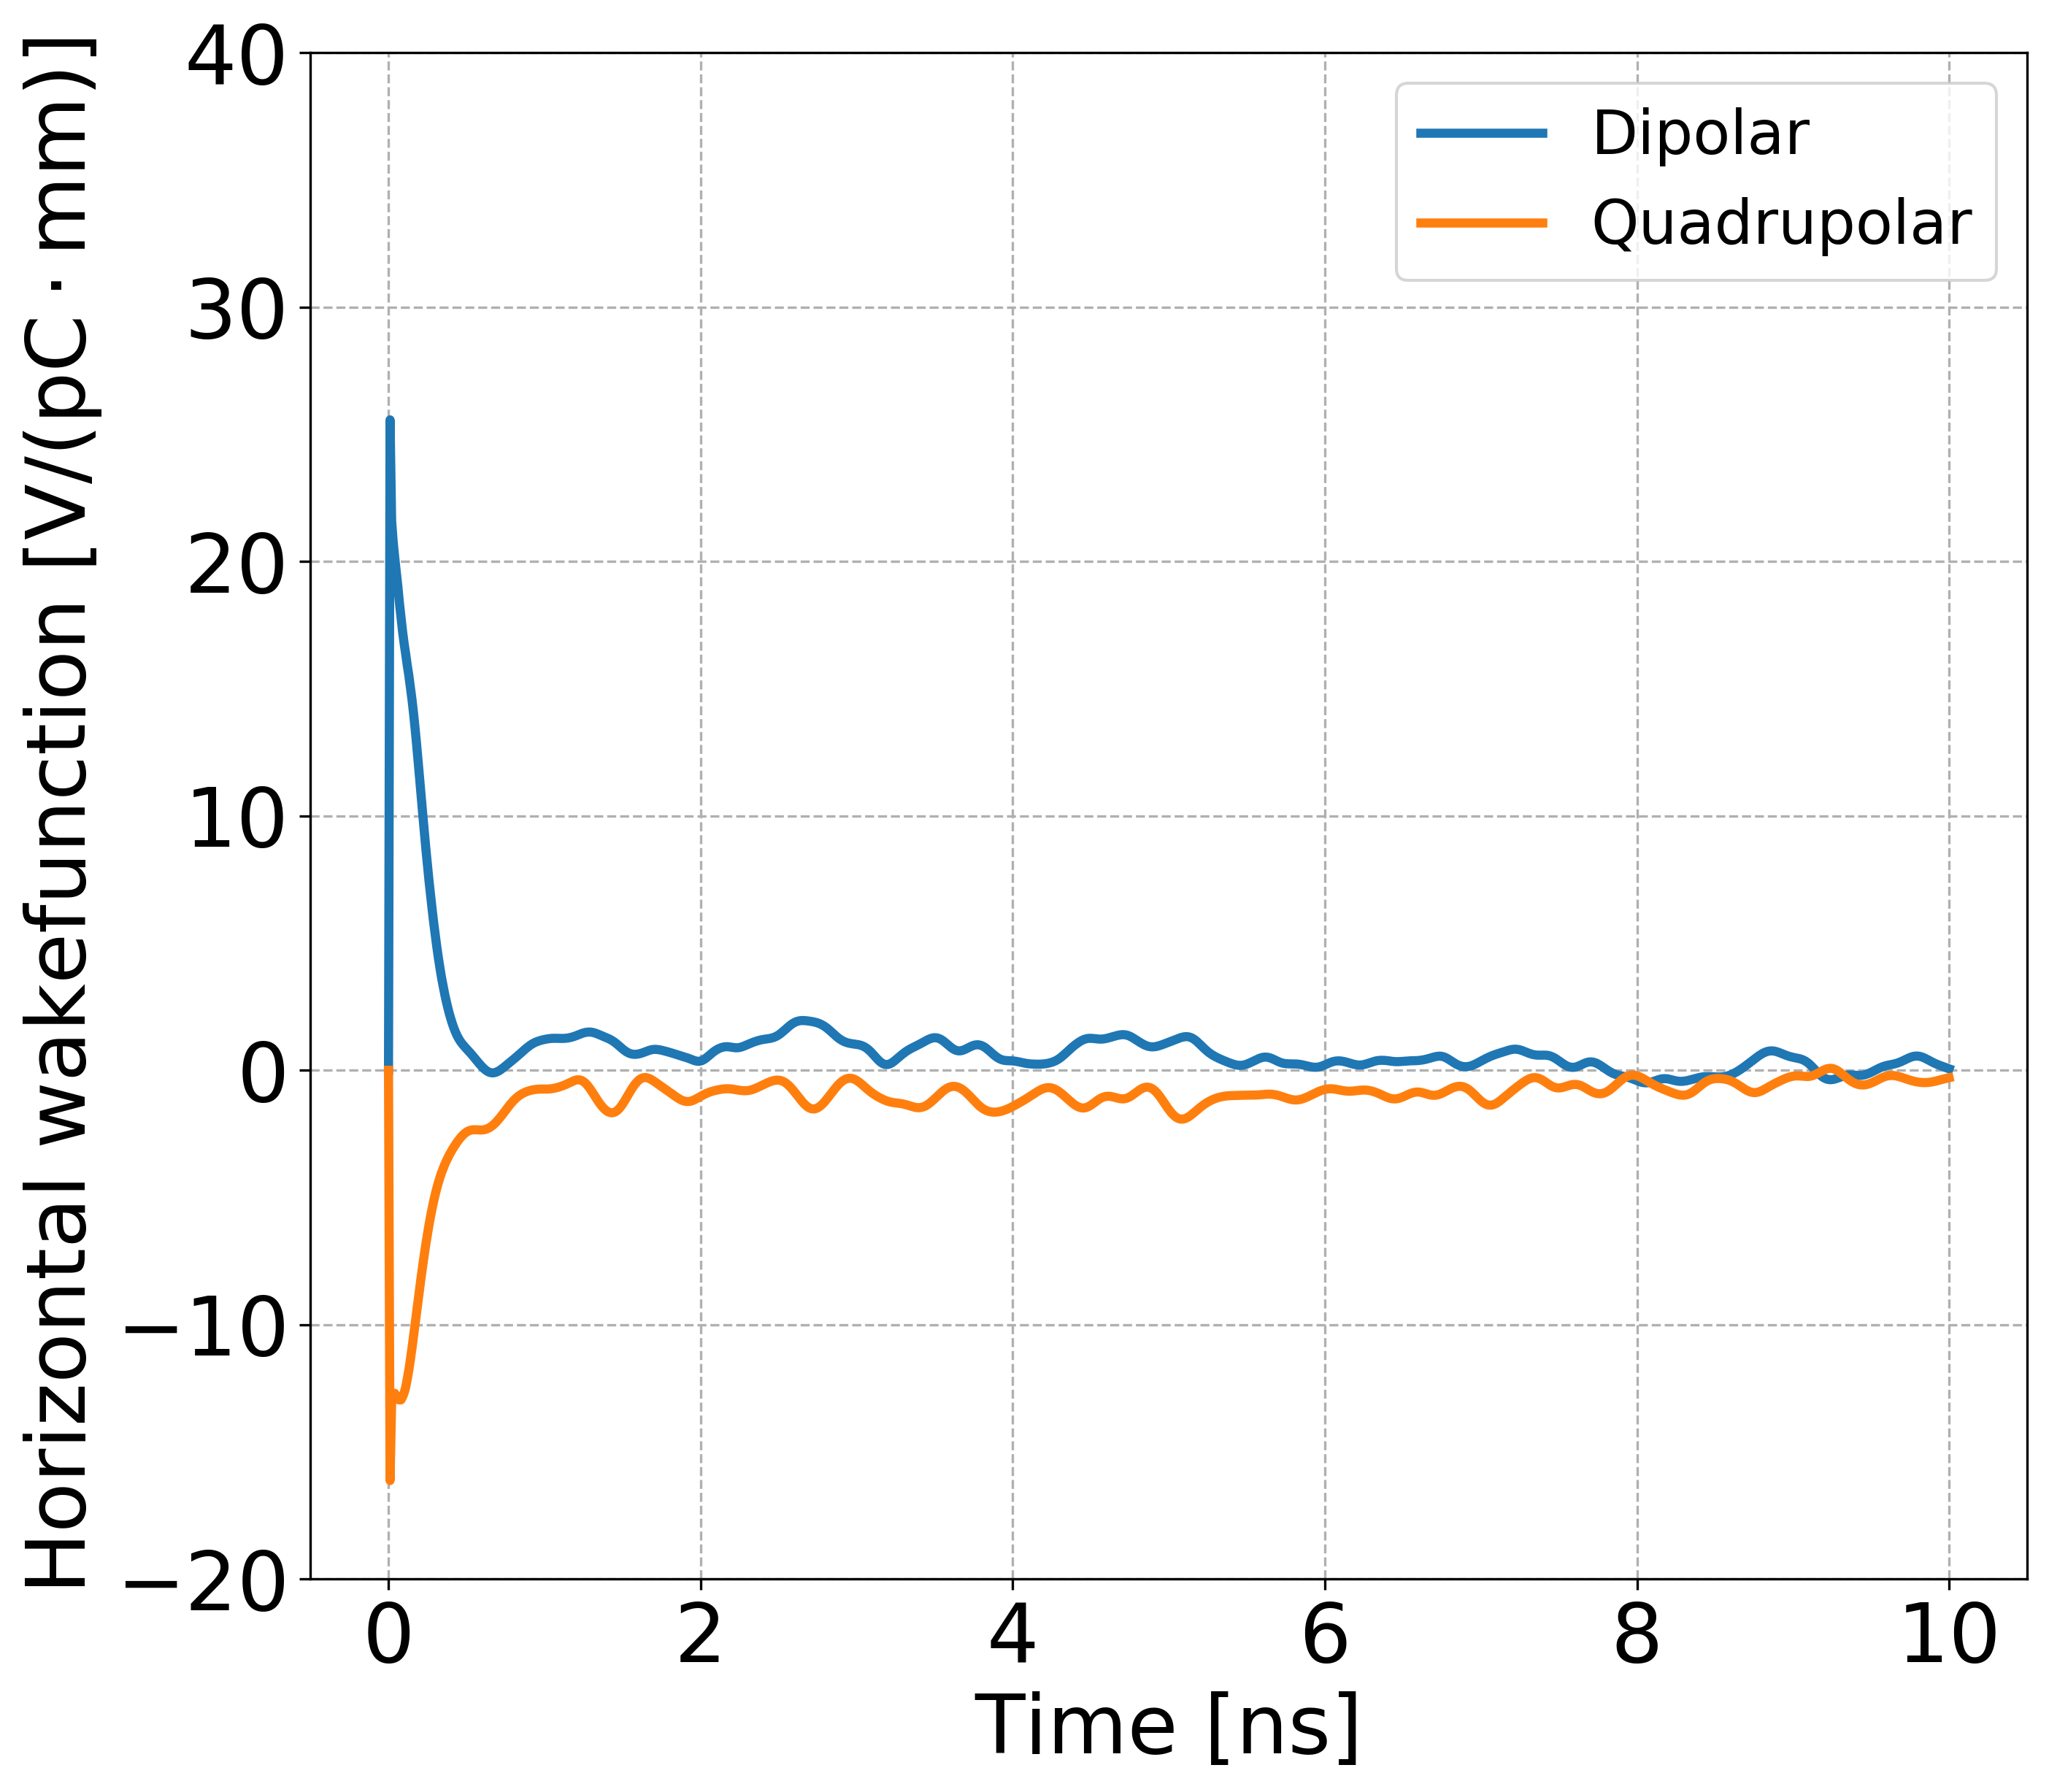
\includegraphics[width=1\textwidth]{images/Ch7/Q26_complete_SPS_model_wakefunctions_H_plane.png}
        %\caption{$y=\sin(2 \pi f t),\ f=50$ Hz}
        %\label{fig:add_label_here}
    \end{subfigure}
    \hfill
    \begin{subfigure}[t]{0.45\textwidth}
        \centering
        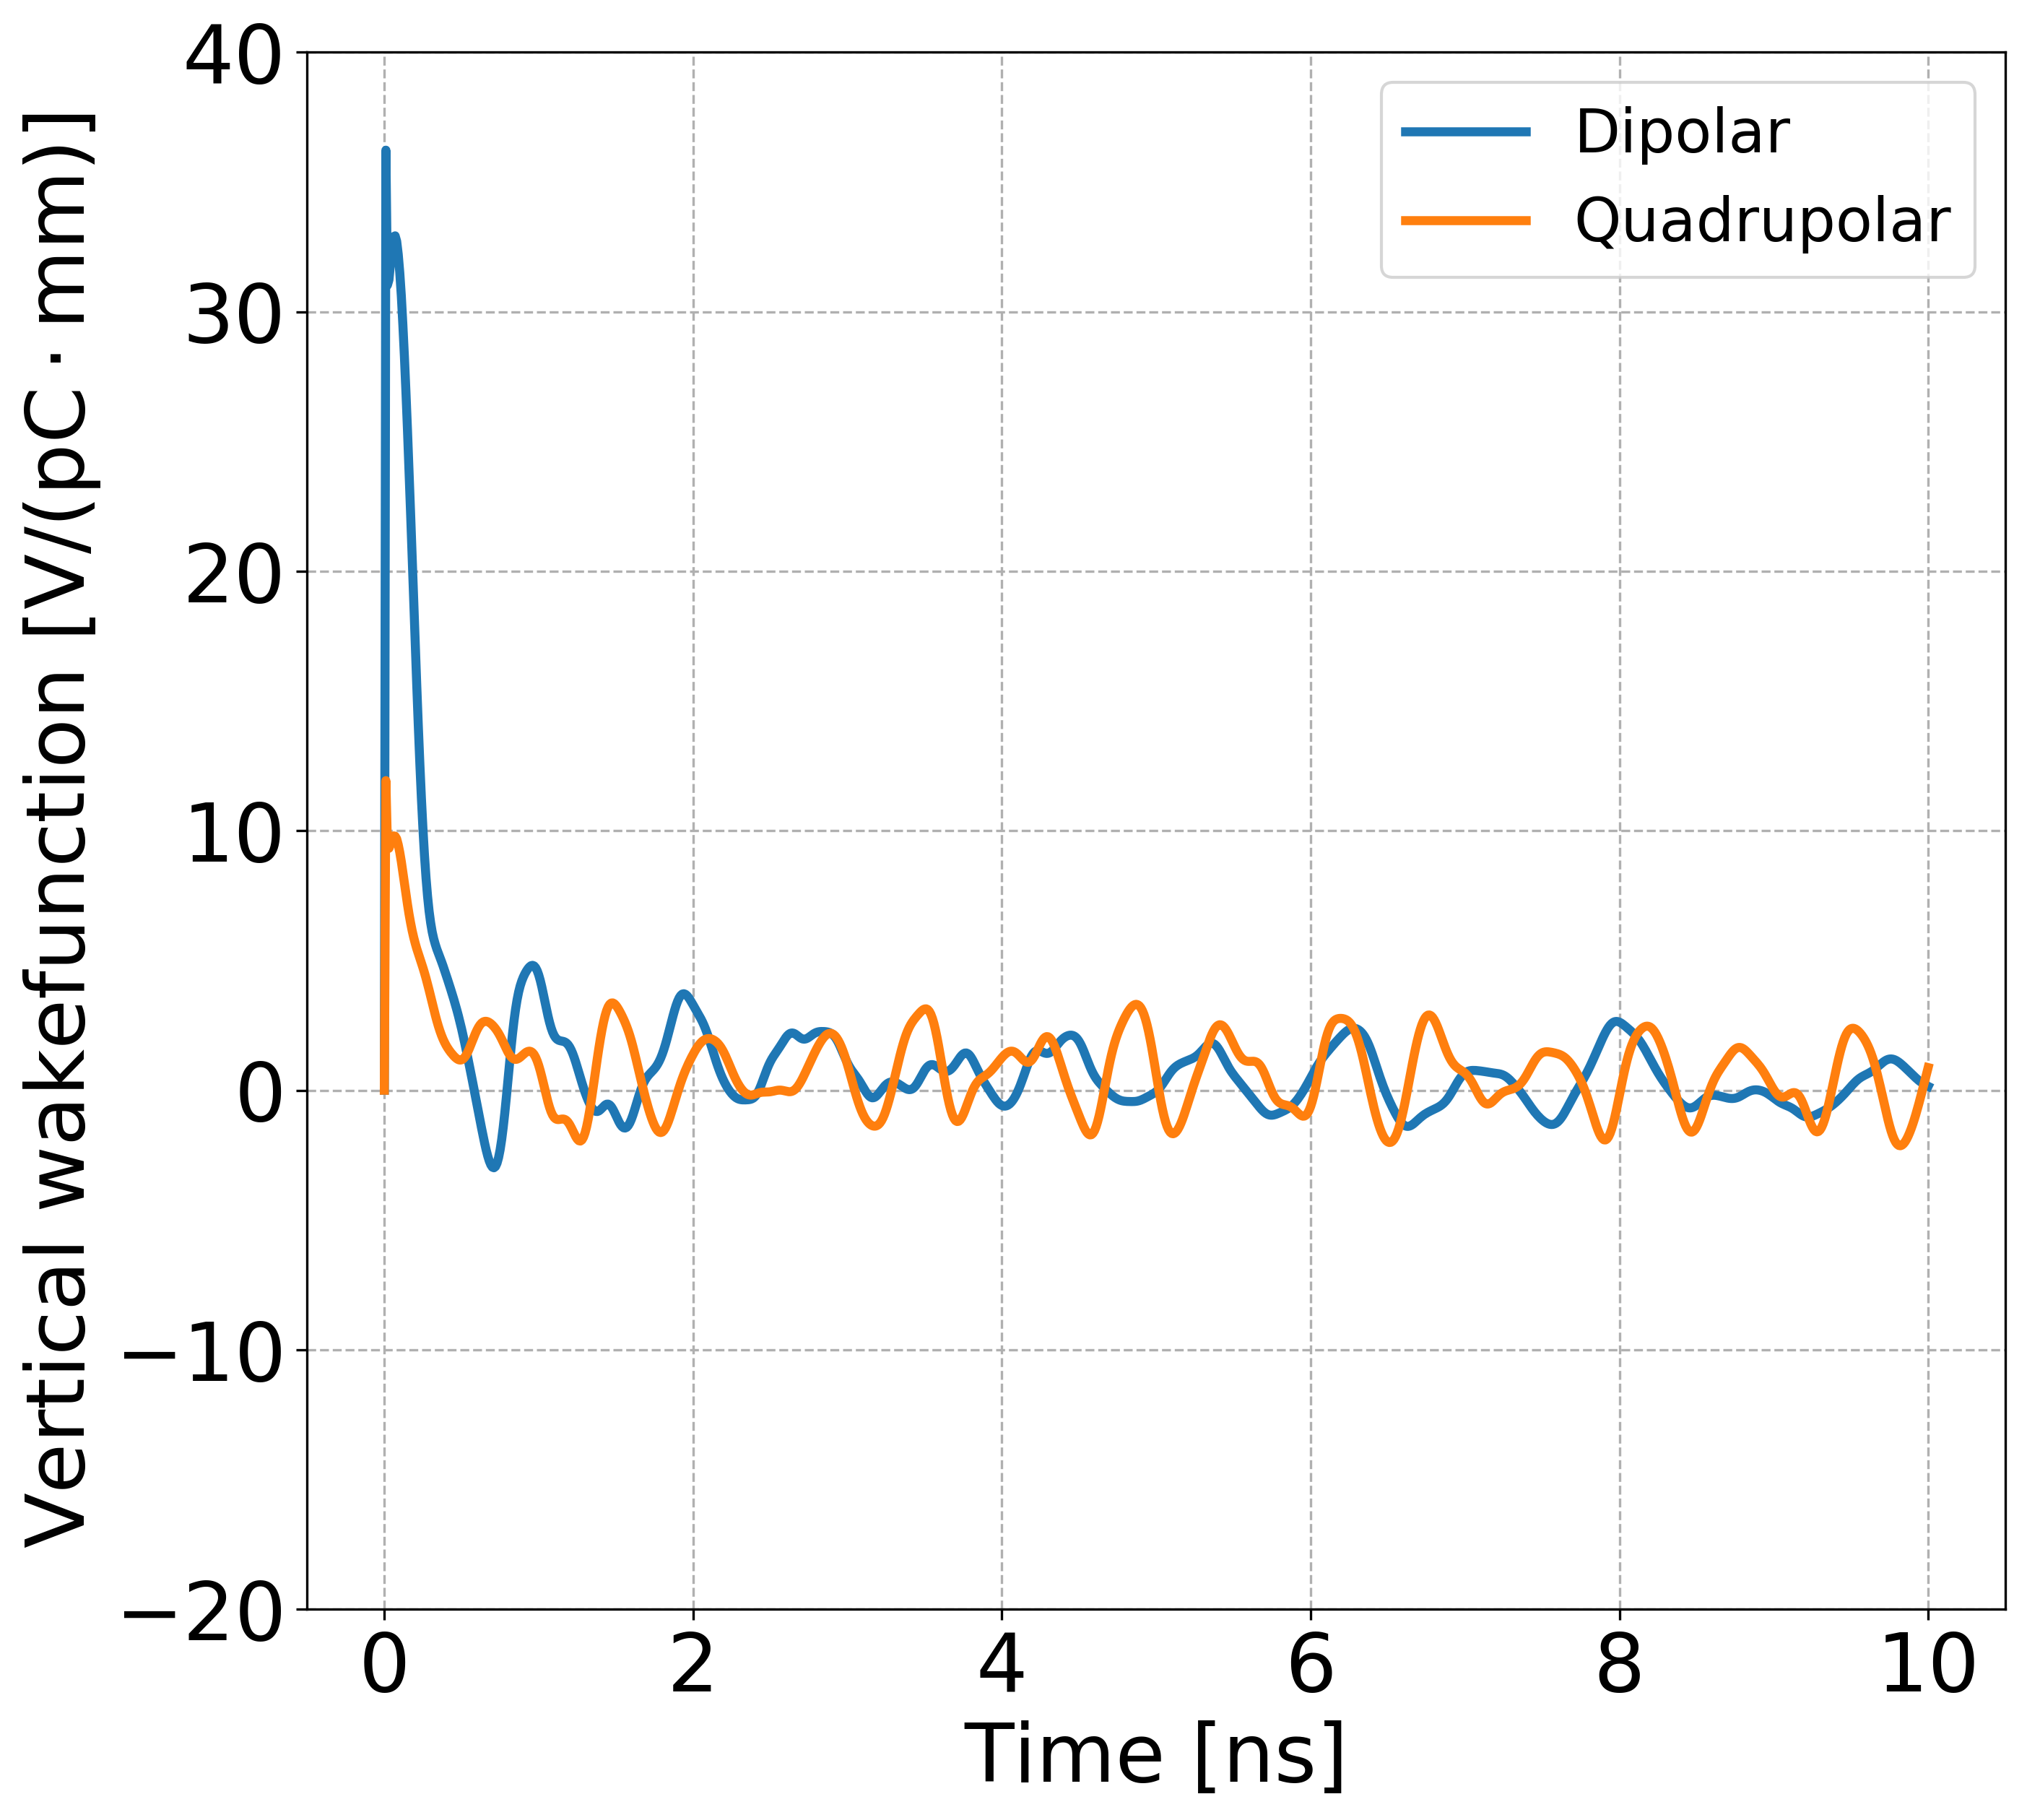
\includegraphics[width=1\textwidth]{images/Ch7/Q26_complete_SPS_model_wakefunctions_V_plane.png}
        %\caption{Discrete Fourier transform}
        %\label{fig:add_label_here}
    \end{subfigure}
    \hfill
     \caption{Horizontal (left) and vertical (right) wakefunctions of the SPS. The wake functions are available in the public gitlab repository of Ref.~\cite{sps_impedance_model_git}. For comparison the bunch length in the SPS CC experiments is $\sim$ 1.85\,ns (4$\mathrm{\sigma_t}$).} % bunch passage
     \label{fig:sps_wakefunctions_model_H_V}
 \end{figure}


% slide 9 https://accelconf.web.cern.ch/ipac2019/talks/weypls1_talk.pdf

% Carlo Zaninni thesis: s, it is important to have an accurate description of the wake at a distance z significantly smaller than the RMS bunch-length, which means that the impedance calculation needs to be accurate up to very high frequency (depending on the accelerator we consider, from a few GHz to the range of THz). 

\subsection{Testing the implementation in PyHEADTAIL}\label{subsec:test_implementation_pyheatail}
As discussed in Section~\ref{subsec:wakefields} the imaginary part of the impedance leads to a coherent tune shift which depends on the bunch intensity. One of the most common ways to test the correct implementation of the impedance model in a tracking simulation code is to benchmark the simulated intensity-dependent coherent tune shift with the theoretically predicted behavior (using Eqs.~\eqref{eq:complext_tune_shift_modes_m} and ~\eqref{eq:real_tunu_mode_l}).

Typically, in tracking simulations, the coherent tune is obtained by applying a frequency analysis technique to the oscillations of the centroid of the particle distribution (the center of mass of the bunch). Here, the analysis is limited to the coherent mode $l=0$ as it can be obtained using a simple Fast Fourier Transform (FFT) algorithm~\cite{FFT_and_applications}. Higher modes (in absolute value, i.e. $l=\pm 1, \pm 2$ etc) can be obtained with more complex algorithms such as the oned provided from the SUSSIX code~\cite{Bartolini:702438} \footnote{The SUSSIX code is applied to the complex position in phase space, $u-i p_u$, while an FFT algorithm is applied only to the transverse position $u$, where $u=(x,y)$~\cite{Salvant:1274254}.}. Nevertheless, the study of mode $l=0$ is sufficient for the purpose of the studies presented here. For simplicity in the following the term "coherent tune" will refer to the coherent tune of mode $l=0$.

In this thesis, the coherent tune is computed using the NAFF algorithm~\cite{LASKAR1990266, Kostoglou:2289645} which provides a refined FFT analysis and its python implementation can be found in the corresponding package in Ref.~\cite{nafflib_repository}.


\textbf{Simulations setup}\\
The parameters used for setting up the linear transfer map, the longitudinal tracking, and the beam initialisation are shown in Table~\ref{tab:pyheadtail_simulation_parameters} and are the ones used in the SPS $\CC$ experiment of 2018. The ring is consisted of one segment, with one interaction point at which the beam interacts with the wakefields. At that location, the horizontal and vertical beta functions equal the corresponding average beta functions over the SPS machine (see Section~\ref{subsec:pyheadtail}). The latest transverse wakefield model (as of February 2019 in Ref~\cite{sps_impedance_model_git}) of the SPS was used.

For the PyHEADTAIL simulation studies presented in this thesis, the Twiss parameter $\alpha_u(s)$ and the dispersion function $D_u(s)$ equal zero. This is a valid assumption for the studies as these parameters have no direct impact on the effects under investigation.

\begin{table}[!hbt]
	\begin{minipage}{\textwidth}
      \begin{centering}
   \caption{PyHEADTAIL simulation parameters used to study impedance induced effects for the SPS.}
	\begin{tabu} to \textwidth {X[c,m] X[0.5c,m] X[0.5c,m] X[0.01c,m]}
		&&& \\[-6mm]
		\toprule \toprule
		\multicolumn{2}{l}{\textbf{Parameter}} &
		\multicolumn{2}{c}{\textbf{Value}} \\
		\bottomrule
      \multicolumn{2}{l}{Beam energy, $\symE$} & \multicolumn{2}{c}{270\,GeV} \\
      \multicolumn{2}{l}{Machine circumference, $C_0$}  & \multicolumn{2}{c}{6911.5623\,kHz} \\
      \multicolumn{2}{l}{Horizontal / Vertical betatron tune, $\Qx$ / $\Qy$}  & \multicolumn{2}{c}{26.13 / 26.18} \\
      \multicolumn{2}{l}{Synchrotron tune, $\Qs$}  & \multicolumn{2}{c}{0.0051}\\
      \multicolumn{2}{l}{Momentum compaction factor, $\alpha_p$}  & \multicolumn{2}{c}{1.9$\cdot 10^{-3}$}\\
      \multicolumn{2}{l}{Number of bunches}  & \multicolumn{2}{c}{1} \\
      \multicolumn{2}{l}{Rms bunch length, 4$\sigmat$}  & \multicolumn{2}{c}{1.7\,ns}\\
      \multicolumn{2}{l}{Horizontal / Vertical normalised emittance, $\epsilon_x$ / $\epsilon_y$}  & \multicolumn{2}{c}{2\,$\mathrm{\mu m}$ / 2\,$\mathrm{\mu m}$}\\
      \multicolumn{2}{l}{Average horizontal / vertical beta function, $\langle \beta_x \rangle / \langle \beta_y \rangle$}  & \multicolumn{2}{c}{42.0941\,m / 42.0137\,m $^\ast$ } \\
      \bottomrule
	\end{tabu}
   \label{tab:pyheadtail_simulation_parameters}
   \end{centering}\footnotesize{$^\ast$ Model values for the Q26 optics.}
   \end{minipage}
\end{table}


- How do you compute the modes.
- Need to give intiial offset.



In particular, the imaginary part of the impedance leads to a real coherent frequency shift (Eq.~\eqref{eq:complext_tune_shift_modes_m}) which can be observed by looking at the Fourier spectrum of the bunch centroid (the center of mass of the bunch) and by comparing it with the unperturbed tune (in the absence of impedance or of other detuning effects).


is to compute the coherent betatron tune as a function of intensity and benchmark it against the theoretically expected values. The rms value of the beta functions over the machine is also listed 

\textbf{Coherent betatron tune from analytical formula}\\
The coherent tune shift due to impedance for a given value of intensity can be computed using the Sacherer formula discussed in Eq.~\eqref{eq:complext_tune_shift_modes_m}. In particular, the coherent frequency shift corresponds to the headtail mode 0. For $l=0$, Eq.~\eqref{eq:complext_tune_shift_modes_m} becomes:
\begin{equation}
    \Omega^{(0)} - \omega_u = - \frac{\sqrt{\pi}}{4 \pi}\frac{N r_0 c^2}{\gamma_0 \frac{2\pi}{\omega_\mathrm{rev}}\omega_u \sigma_z} i Z_\mathrm{eff}.
\end{equation}
Replacing $Q_u = \omega_u/\omega_\mathrm{rev}$, where $u=(x,y)$, in the above equation gives:
\begin{equation}\label{eq:complex_tune_shfit_for_coherent_mode}
    \Delta \Omega^{(0)} = - \frac{N r_0 c^2}{8 \pi^{3/2} \gamma_0 Q_u \sigma z} i Z_\mathrm{eff}.
\end{equation}
All the parameters inserted in Eq.~\eqref{eq:complex_tune_shfit_for_coherent_mode} should be converted in CGS (centimetre–gram–second) units.
Then the coherent betatron tune shift is computed as:
\begin{equation}
    \Delta Q_u = \frac{\Delta \Omega^{(0)}}{\omega_\mathrm{rev}}.
\end{equation}

\textbf{Coherent betatron tune from PyHEADTAIL simulations}\\
   \label{tab:pyheadtail_simulation_parameters}
The coherent tune is defined as the frequency of the transverse oscillations of the centroid.
Typically, in tracking simulations the coherent tune can be obtained by applying an FFT algorithm on the motion of the centroid.


The coherent tune can be obtained by tracking simulation 



The PyHEADTAIL simulations were performed for the parameters used in the SPS $\CC$ experiment in 2018 as shown in Table~\ref{tab:pyheadtail_simulation_parameters}. The average transverse beta functions over the SPS are also listed, as they are used for the implementation of the wakefields in the simulations (see Section~\ref{subsec:pyheadtail} ).The latest transverse wakefield model (as of February 2019 in Ref~\cite{sps_impedance_model_git}) of the SPS was used.







- growth rate of mode 0
- shift of mode 0
One of the properties which is also used for checking the correct implemetation of the model. which as we will say later on is relevant to the suppression mechanism is the coherent tune shift with 

- model benchmarked but not as thorough for ... not gor single bunhces at that low intensity?

- we figured out


\section{Setting up emittance growth simualtions}
The setup of the PyHEADTAIL simulations that were performed to study the impact of the beam coupling impedance on the emittance growth due to $\CC$ RF noise was done following the steps described in Section~\ref{subsec:pyheadtail}. The relevant machine and beam parameters are summarised in Table~\ref{tab:sps_pyheadtail_emit_growth_parameters}


This section describes the setup of the PyHEADTAIL simulations that were performed to study the impact of the beam coupling impedance on the emittance growth due to $\CC$ RF noise. The machine and beam initialisation


From M . schenk
PYHEADTAIL employs the detuning implementation of the octupole magnets where
every particle receives, instead of transverse kicks, amplitude-dependent changes to its phase advances in order to model the incoherent tune shifts



. The optics parameters were extracted from the SPS design parameters (nominal model for Q26 optics: Section~\ref{subsec:SPS_optics_model}), excpet for the vertical alpha function at the location of the CC2, $\alpha_{y, CC2}$ which is set to zero for simplicity as its value doesn't affect the emittance evolution. \textcolor{red}{Maybe elaborate a bit more on why it doesn't affect it?}. The rest of the listed parameters were chosen to be very close to the experimental conditions during the emittance growth measurements of 2018 (discussed in Chapter~\ref{Ch:2018_analyisis}).


\begin{table}[!hbt]
	\begin{minipage}{\textwidth}
      \begin{centering}
   \caption{Relevant machine and beam parameters used to study the impact of the beam transverse impedance on the emittance evolution due to CC RF noise with the PyHEADTAIL code.}
	\begin{tabu} to \textwidth {X[c,m] X[0.5c,m] X[0.5c,m] X[0.01c,m]}
		&&& \\[-6mm]
		\toprule \toprule
		\multicolumn{2}{l}{\textbf{Parameter}} &
		\multicolumn{2}{c}{\textbf{Value}} \\
		\bottomrule
      \multicolumn{2}{l}{Beam energy, $\symE$} & \multicolumn{2}{c}{270\,GeV} \\
      \multicolumn{2}{l}{Number of protons per bunch, $\Nb$} & \multicolumn{2}{c}{3 $\times 10^{10}$ p/b} \\
      \multicolumn{2}{l}{Horizontal / Vertical betatron tune, $\Qx$ / $\Qy$}  & \multicolumn{2}{c}{26.13 / 26.18} \\
      \multicolumn{2}{l}{Horizontal / Vertical first order chromaticity, $\Qpx$ / $\Qpy$}  & \multicolumn{2}{c}{1 / 1} \\
      \multicolumn{2}{l}{Main RF voltage / frequency,  $\VRF$ / $\fRF$}  & \multicolumn{2}{c}{5.088\,MV / 200.39\,MHz} \\ %200.3945
      \multicolumn{2}{l}{Synchrotron tune, $\Qs$}  & \multicolumn{2}{c}{0.0051} \\
      \multicolumn{2}{l}{$\CC 2$ voltage / frequency, $\VCC $ / $\fCC$}  & \multicolumn{2}{c}{1\,MV / 400.78\,MHz} \\
      \multicolumn{2}{l}{Vertical beta function at $\CC 2$, $\beta_{y, CC2}$}  & \multicolumn{2}{c}{73.82\,m} \\
      \multicolumn{2}{l}{Vertical alpha function at $\CC 2$, $\alpha_{y, CC2}$}  & \multicolumn{2}{c}{0\,m} \\
      \multicolumn{2}{l}{Vertical dispersion at $\CC 2$, $D_{y, CC2}$}  & \multicolumn{2}{c}{0\,m} \\
      \multicolumn{2}{l}{Number of bunches}  & \multicolumn{2}{c}{1} \\
      \multicolumn{2}{l}{Rms bunch length, 4$\sigmat$}  & \multicolumn{2}{c}{1.8 \,ns$^\ast$}\\
      \multicolumn{2}{l}{Horizontal / Vertical normalised emittance, $\emitx$ / $\emity$}  & \multicolumn{2}{c}{2\,$\mathrm{\mu m}$ / 2\,$\mathrm{\mu m^\ast}$}\\
      \multicolumn{2}{l}{Horizontal / Vertical rms tune spread, $\Dqxrms$ / $\Dqyrms$}  & \multicolumn{2}{c}{2.02 $\times 10^{-5}$ / 2.17 $\times 10^{-5}$ $^\dagger$}\\
      \bottomrule
	\end{tabu}
   \label{tab:sps_pyheadtail_emit_growth_parameters}
   \end{centering} \footnotesize{$^\ast$ Initial values at the beginning of the tracking.\\$^\dagger$ Here the rms betatron tune spread includes only the contribution from the detuning with amplitude present in the SPS machine. More details along with the calulcations for the listed values can be found in Appendix~\ref{app:detuning_with_amplitude}.}
   \end{minipage}
\end{table}

\normalsize{\textbf{Crab Cavity RF noise levels}}\\
For the simulation studies presented in this chapter, the phase and amplitude noise are modeled as random kicks on the particles' momentum according to the work of T. Mastoridis and P. Baudrenghien in Ref~\cite{PhysRevSTAB.18.101001}, as follows:
\begin{equation}
    \mathrm{\textbf{Phase \ noise:}} \ y^\prime_{i,1} = y^\prime_{i, 0} + A \cos{\left ( \frac{2\pi \fCC}{c \betarel}z_i \right )},
\end{equation}

\begin{equation}
    \mathrm{\textbf{Amplitude \ noise:}} \ y^\prime_{i, 1} = y^\prime_{i, 0} + A \sin{\left ( \frac{2\pi \fCC}{c \betarel}z_i \right )},
\end{equation}

where $i=1...N$ with being $N$ the number of macroparticles used in the simulation,  $\fCC$ is the $\CC$ frequency in Hz, $c$ is the speed of light in m/s, $\betarel$ the relativistic beta and $z_i$ the longitudinal position of each particle in m. The factor $A=\VCC$
%slide 5: https://docs.google.com/presentation/d/1Jv0Es99utlZSSg25_9oplI53A5MdPDfJSjsSneRXaV8/edit#slide=id.gbb99f3cf0a_0_65




\normalsize{\textbf{Amplitude detuning}}\\
\normalsize{\textbf{Parameters particularly for simulations without imepdance effects}}\\
\normalsize{\textbf{Parameters particularly for simulations with imepdance effects}}\\


The parameters used for the simulations were

imulations used the SPS design parameters and the beam conditions as in the experiment of 2018.

Table with parameters, including macroparticles number + slices + average beta funtion for convinience.




\section{First observations of emittance growth suppression by the impedance}


\section{Characterisation of the emittance growth suppression by the impedance}

\section{Suppresion mechanism}\label{sec:suppression_mechanism}
\subsection{Past studies with beam-beam interactions}\label{subsec:past_studies_impedance_suppression_BB}
\subsection{Intensity scans}
\subsection{Schottky noise spectra}
